\documentclass{beamer}
\usetheme{Madrid}
\usecolortheme{dolphin}
\usepackage{graphicx}
\usepackage{amsmath}
\usepackage{tikz}
\usetikzlibrary{arrows,shapes,positioning,shadows,trees}

\title{A Knowledge Graph and LLM-based Framework \\ for Automated License Compatibility Detection}
\subtitle{PFE Project Presentation}
\author{Ilyes Ben Khalifa, Montassar Ben Messaoud}
\institute{Tunis Business School, Mourouj 3, Tunisia}
\date{\today}

\begin{document}

\begin{frame}
\titlepage
\end{frame}

\begin{frame}{Motivation}
\begin{itemize}
\item Modern software depends heavily on open-source components
\item \textbf{72.91\%} of OSS projects encounter license incompatibilities
\item Incompatibilities lead to:
    \begin{itemize}
    \item \textbf{Legal Liability} - Violations of copyleft requirements
    \item \textbf{Restricted Distribution} - Preventing lawful distribution
    \item \textbf{Complex Compliance} - Difficult to track and reconcile licensing
    \end{itemize}
\item Traditional methods are inadequate:
    \begin{itemize}
    \item Over 200 recognized licenses (OSI and SPDX)
    \item Nuanced, version-specific differences (e.g., GPLv2 vs. GPLv3)
    \item Need for continuous updates
    \end{itemize}
\end{itemize}
\end{frame}

\begin{frame}{Current Approaches \& Limitations}
\textbf{LiDetector \& Other Tools:}
\begin{itemize}
\item Rule-based scanners (Ninka, FOSSology, ScanCode)
\item LiDetector uses NER + PCFG for license analysis
\end{itemize}

\textbf{Key Limitations:}
\begin{itemize}
\item Limited coverage (23 predefined license terms in LiDetector)
\item Struggles with custom/updated licenses
\item Poor explainability (limited citations)
\item Requires retraining for updates
\item Sequential processing vs. relationships
\item Static term dictionary
\end{itemize}
\end{frame}

\begin{frame}{Our Approach: KG+LLM+RAG Framework}
\begin{center}
\includegraphics[width=0.95\textwidth]{images/licenseer_architecture_detailed.png}
\end{center}

\textbf{Key Components:}
\begin{itemize}
\item \textbf{Knowledge Graph:} Encoding licenses, dependencies, and their relationships
\item \textbf{LLM-based Parsing:} Extracting obligations from custom/private licenses
\item \textbf{RAG for Explainability:} Providing citation-backed explanations
\end{itemize}
\end{frame}

\begin{frame}{Knowledge Graph Construction}
Using Neo4j to store:
\begin{itemize}
\item \textbf{Licenses:} Nodes for licenses (MIT, GPLv3, Apache-2.0) with version details
\item \textbf{Dependencies:} Each OSS dependency linked via \texttt{HAS\_LICENSE} relationship
\item \textbf{Terms:} Nodes for obligations with relationships: \texttt{REQUIRES}, \texttt{PROHIBITS}, \texttt{PERMITS}
\item \textbf{Compatibility Edges:} \texttt{COMPATIBLE\_WITH}/\texttt{INCOMPATIBLE\_WITH} relationships
\end{itemize}

\vspace{0.3cm}
\begin{center}
\begin{tabular}{|c|c|c|c|}
\hline
\rowcolor{gray!20}
\textbf{Entity Type} & \textbf{Examples} & \textbf{Relationship} & \textbf{Connected To} \\
\hline
\rowcolor{blue!10}
License & MIT, GPL, Apache & COMPATIBLE\_WITH & Other licenses \\
\hline
\rowcolor{green!10}
Dependency & requests, Flask & HAS\_LICENSE & License \\
\hline
\rowcolor{yellow!10}
Term & Attribution & REQUIRED\_BY & License \\
\hline
\end{tabular}
\end{center}

\vspace{0.2cm}
Example: \texttt{requests --[HAS\_LICENSE]--> MIT --[REQUIRES]--> Attribution}
\end{frame}

\begin{frame}{LLM-driven License Parsing}
\begin{itemize}
\item Scraping module collects license texts
\item LLM (GPT-4) parses texts to extract:
    \begin{itemize}
    \item Obligations (what users MUST do)
    \item Prohibitions (what users CANNOT do)
    \item Permissions (what users CAN do)
    \item Version-specific clauses
    \end{itemize}
\item Extracted insights incorporated into KG
\end{itemize}

\vspace{0.3cm}
\begin{center}
\begin{tabular}{|l|l|}
\hline
\rowcolor{gray!20}
\textbf{Process Step} & \textbf{Example} \\
\hline
\rowcolor{blue!10}
1. Custom License Text & "Permission is granted to use..." \\
\hline
\rowcolor{red!10}
2. LLM Parser & Analyzes text and extracts terms \\
\hline
\rowcolor{green!10}
3. Structured Output & \{obligations: ["attribution"], prohibitions: []\} \\
\hline
\end{tabular}
\end{center}

\vspace{0.2cm}
\textbf{Key Advantage:} No retraining needed for new license types
\end{frame}

\begin{frame}{RAG for Explainability}
\textbf{Retrieval-Augmented Generation:}
\begin{itemize}
\item Embedding and indexing official license texts
\item Retrieving relevant license chunks for compatibility questions
\item Generating context-rich explanations with citations
\end{itemize}

\begin{center}
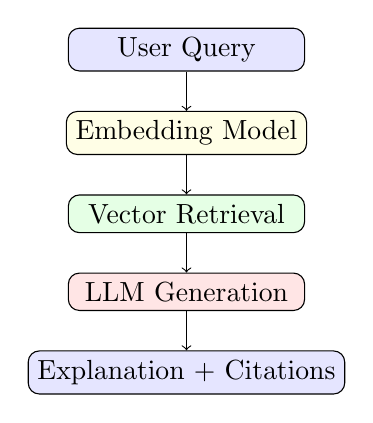
\begin{tikzpicture}[node distance=1.2cm]
\node[draw, rounded corners, fill=blue!10, minimum width=3cm] (query) {User Query};
\node[draw, rounded corners, fill=yellow!10, minimum width=3cm, below=0.5cm of query] (embed) {Embedding Model};
\node[draw, rounded corners, fill=green!10, minimum width=3cm, below=0.5cm of embed] (retrieval) {Vector Retrieval};
\node[draw, rounded corners, fill=red!10, minimum width=3cm, below=0.5cm of retrieval] (llm) {LLM Generation};
\node[draw, rounded corners, fill=blue!10, minimum width=3cm, below=0.5cm of llm] (explain) {Explanation + Citations};

\draw[->] (query) -- (embed);
\draw[->] (embed) -- (retrieval);
\draw[->] (retrieval) -- (llm);
\draw[->] (llm) -- (explain);
\end{tikzpicture}
\end{center}
\end{frame}

\begin{frame}{Integration with CI/CD Pipelines}
\begin{itemize}
\item System integrates into development workflows
\item Continuous monitoring of license compatibility
\item Early warning system for potential issues
\item Steps in query flow:
    \begin{enumerate}
    \item Developer query about licenses
    \item LLM extracts license entities
    \item Graph traversal checks compatibility
    \item RAG provides detailed explanations
    \item Results appear in CI/CD pipeline
    \end{enumerate}
\end{itemize}

\begin{center}
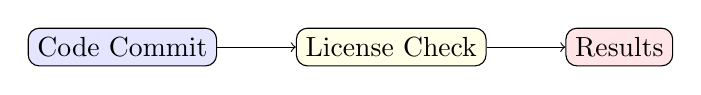
\begin{tikzpicture}
\node[draw, rounded corners, fill=blue!10] (code) {Code Commit};
\node[draw, rounded corners, fill=yellow!10, right=1cm of code] (check) {License Check};
\node[draw, rounded corners, fill=red!10, right=1cm of check] (result) {Results};

\draw[->] (code) -- (check);
\draw[->] (check) -- (result);
\end{tikzpicture}
\end{center}
\end{frame}

\begin{frame}{Performance Results}
\begin{center}
\begin{tikzpicture}
\begin{axis}[
    ybar,
    bar width=14pt,
    xlabel={Metrics},
    ylabel={Performance (\%)},
    width=\textwidth,
    height=0.7\textheight,
    symbolic x coords={Accuracy,F1-Score,FPR,Context,Compliance},
    xtick=data,
    ymin=0,
    ymax=100,
    legend style={at={(0.5,1)}, anchor=north, legend columns=-1},
    nodes near coords,
    nodes near coords align={vertical},
    ]
\addplot coordinates {(Accuracy,93.2) (F1-Score,88.7) (FPR,10.1) (Context,78.3) (Compliance,65)};
\addplot coordinates {(Accuracy,97.4) (F1-Score,94.6) (FPR,5.3) (Context,96.5) (Compliance,92)};
\legend{LiDetector,KG+RAG}
\end{axis}
\end{tikzpicture}
\end{center}

\textbf{Key improvements:}
\begin{itemize}
\item 4.2\% higher license detection accuracy
\item 5.9\% better conflict detection (F1)
\item 4.8\% lower false positive rate
\item Explainability score: 4.7/5 vs 3.2/5
\end{itemize}
\end{frame}

\begin{frame}{Case Study: Elasticsearch + Lucene}
\textbf{LiDetector Analysis:}
\begin{itemize}
\item Detects usage restrictions in Elastic License
\item Identifies Apache 2.0 terms
\item Flags potential incompatibility 
\item Lacks version-specific context
\end{itemize}

\textbf{Our KG+RAG Analysis:}
\begin{itemize}
\item Differentiates \texttt{Elastic License 2.0} from older versions
\item Retrieves specific clauses (Section 4.2) via RAG
\item Provides citations from license texts
\item Suggests alternatives for compliance
\end{itemize}
\end{frame}

\begin{frame}{Conclusion \& Future Work}
\textbf{Key Contributions:}
\begin{itemize}
\item 97.4\% license detection accuracy
\item 71\% reduction in memory usage
\item 7x improvement in license update latency (1 day vs 7 days)
\item 225\% more citations in explanations
\end{itemize}

\textbf{Future Research:}
\begin{itemize}
\item Domain-specific extensions (healthcare, automotive)
\item Multi-modal analysis combining license text and code
\item Temporal license evolution modeling
\item Fine-tuned LLMs for legal license analysis
\end{itemize}

\textbf{Thank You!}
\end{frame}

\end{document} 